\documentclass{beamer}
\usetheme{Frankfurt}

\usepackage{listings}

\setbeamertemplate{footline}[frame number]

\newcommand{\todo}[1]{\alert{TODO #1}}

\title{Denial of Service}
\subtitle{Lecture 9 \\ Computer Security DD2395}
\author[R. Guanciale]{
  Roberto Guanciale\\
  robertog@kth.se
}
\date{2015-11-26}
\begin{document}

\begin{frame}[plain]
  \titlepage
\end{frame}

\begin{frame}{Lab W}
  \begin{itemize}
  \item Instructions on-line
  \item Booking for help sessions on-line
  \item All sessions can also be used to report your result
  \item Start tomorrow, go to the lab and start your assignment
  \item Session Dec 17 is only to report you work
  \end{itemize}
\end{frame}

\begin{frame}{Denial of Service}
  \begin{itemize}
  \item denial of service (DoS) an action that prevents or 
    impairs the authorized use of networks, systems, or 
    applications by exhausting resources such as central 
    processing units (CPU), memory, bandwidth, and 
    disk space 
  \item  attacks 
  \begin{itemize}
    \item  network bandwidth 
    \item  system resources 
    \item  application resources 
  \end{itemize}
  \item  have been an issue for some time
  \end{itemize}
\end{frame}

\begin{frame}{Classic Denial of Service Attacks}
  \begin{itemize}
  \item  can use simple flooding ping 
  \item  from higher capacity link to lower 
  \item  causing loss of traffic 
  \item  source of flood traffic easily identified
  \end{itemize}
\end{frame}

\begin{frame}{Classic Denial of Service Attacks}
  \begin{center}
    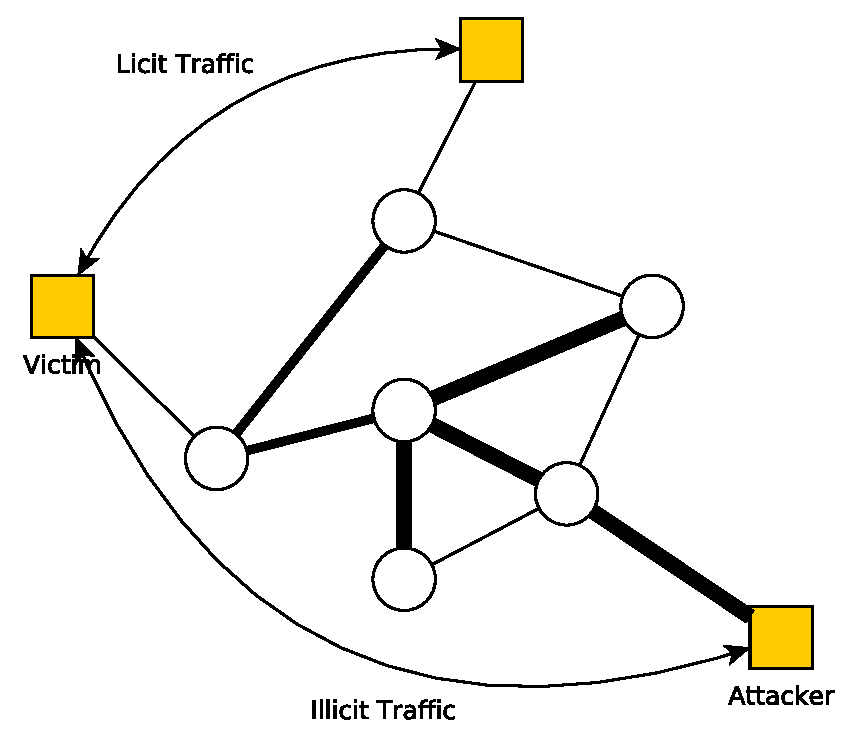
\includegraphics[width=0.8\linewidth]{dos1}
  \end{center}
\end{frame}

\begin{frame}{Source Address Spoofing }
  \begin{itemize}
  \item  use forged source addresses 
    \begin{itemize}
    \item  given sufficient privilege to “raw sockets” 
    \item  easy to create 
    \end{itemize}
  \item  generate large volumes of packets 
  \item  directed at target 
  \item  with different, random, source addresses
  \end{itemize}
\end{frame}



\begin{frame}{Source Address Spoofing }
  \begin{itemize}
  \item Why would an attacker bother doing that?
  \item<2-> To hide his identity
  \item<3-> To avoid back traffic
  \begin{center}
    \includegraphics[width=0.8\linewidth]{dos2}
  \end{center}
  \end{itemize}
\end{frame}

\begin{frame}{Source Address Spoofing }
  \begin{itemize}
  \item Why would an attacker bother doing that?
  \item To hide his identity
  \item To avoid back traffic
  \item IMCP Answers increase the victim's congestion
  \begin{center}
    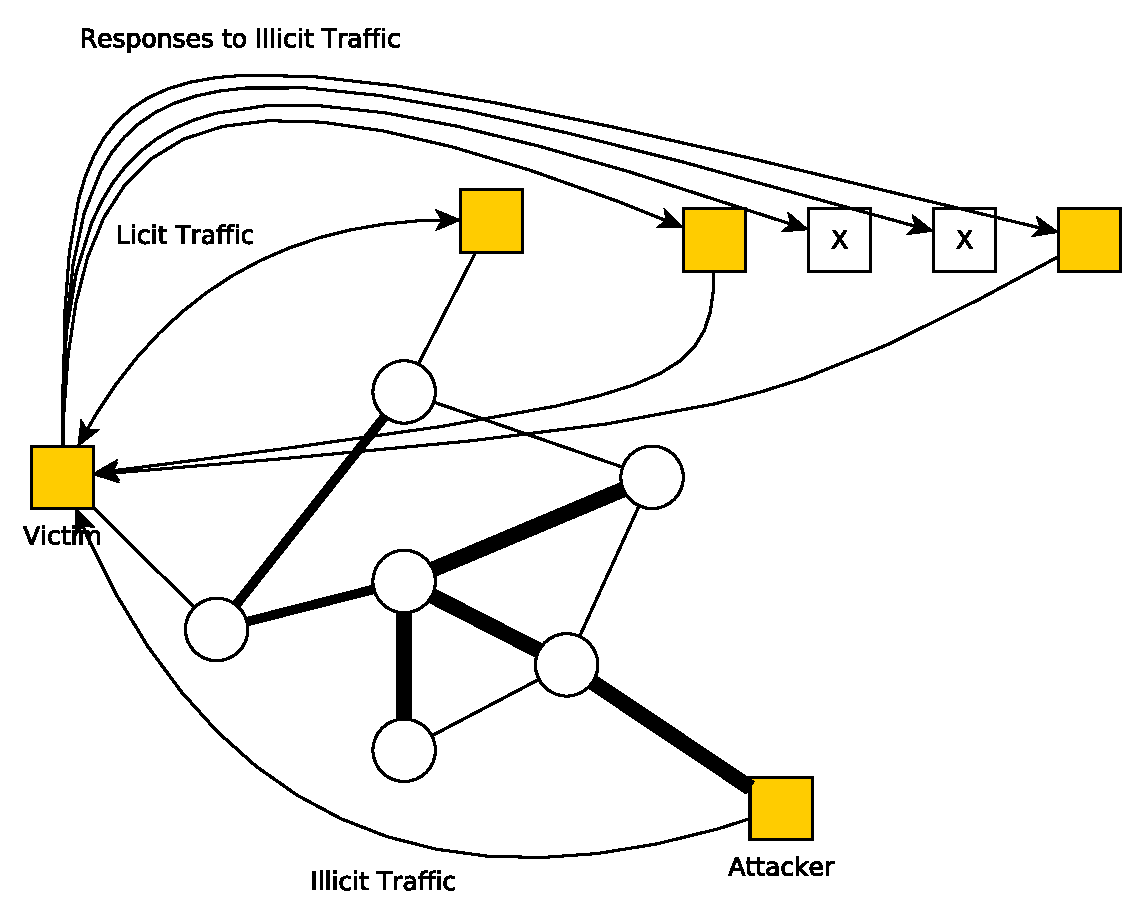
\includegraphics[width=0.7\linewidth]{dos3}
  \end{center}
  \end{itemize}
\end{frame}

\begin{frame}{Source Address Spoofing }
  \begin{itemize}
  \item Why would an attacker bother doing that?
  \item To hide his identity
  \item To avoid back traffic
  \item IMCP Answers increase the victim's congestion
  \item IMCP Answers can be used to identify attacks
  \begin{center}
    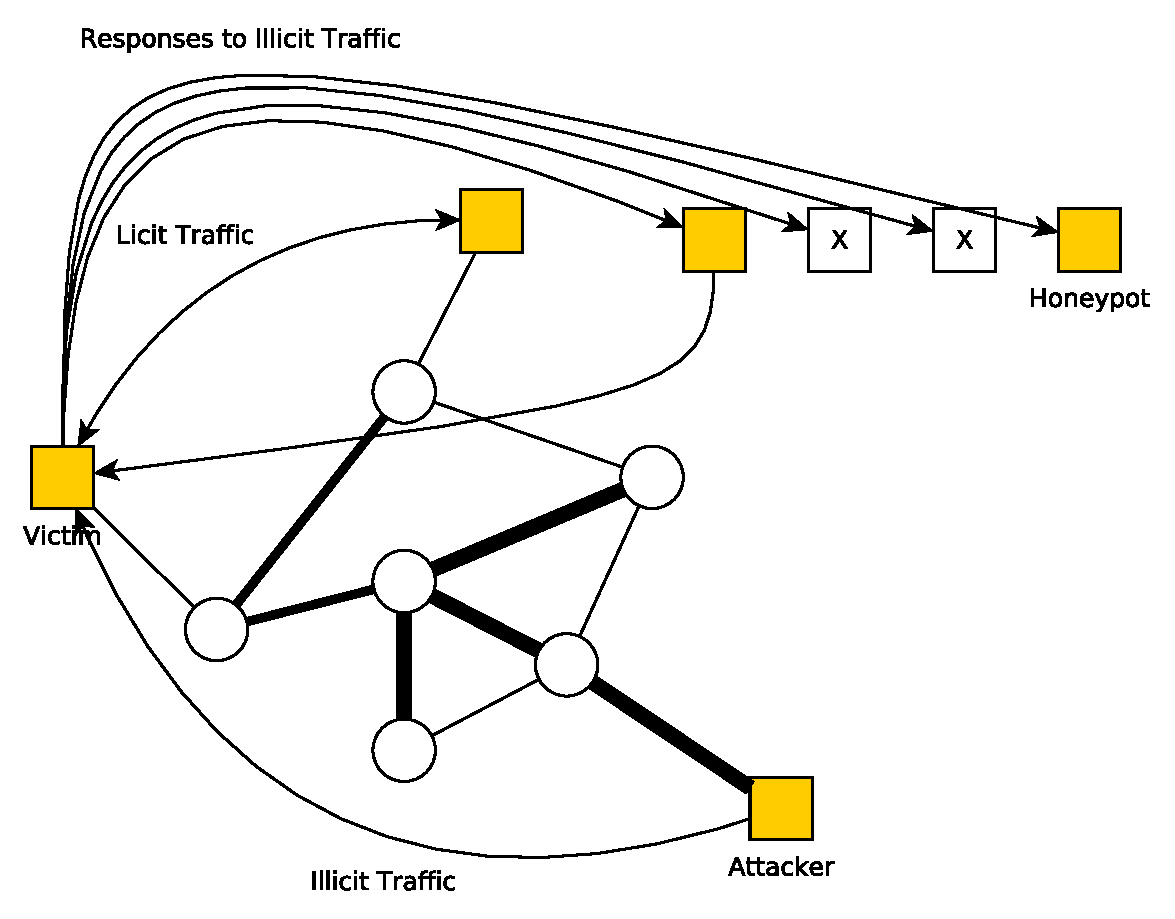
\includegraphics[width=0.6\linewidth]{dos4}
  \end{center}
  \end{itemize}
\end{frame}

\begin{frame}{SYN Spoofing }
  \begin{itemize}
  \item  other common attack 
  \item  attacks ability of a server to respond to future 
    connection requests 
  \item  overflowing tables used to manage them 
  \item  hence an attack on system resource
  \end{itemize}
\end{frame}


\begin{frame}{TCP Connection Handshake}
  \begin{center}
    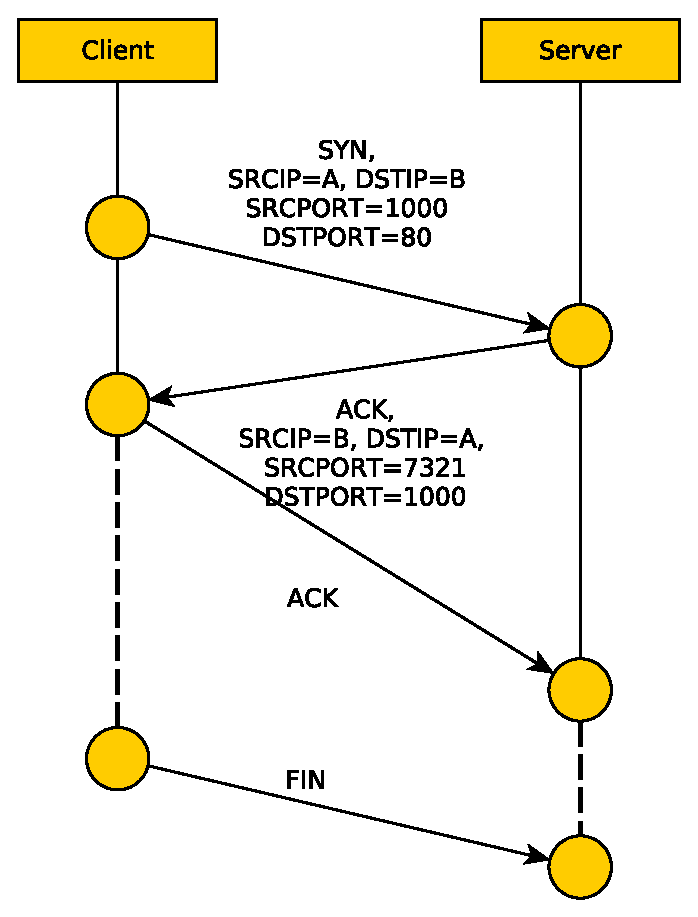
\includegraphics[width=0.5\linewidth]{syn1}
  \end{center}
\end{frame}

\begin{frame}{SYN Spoofing Attack}
  \begin{center}
    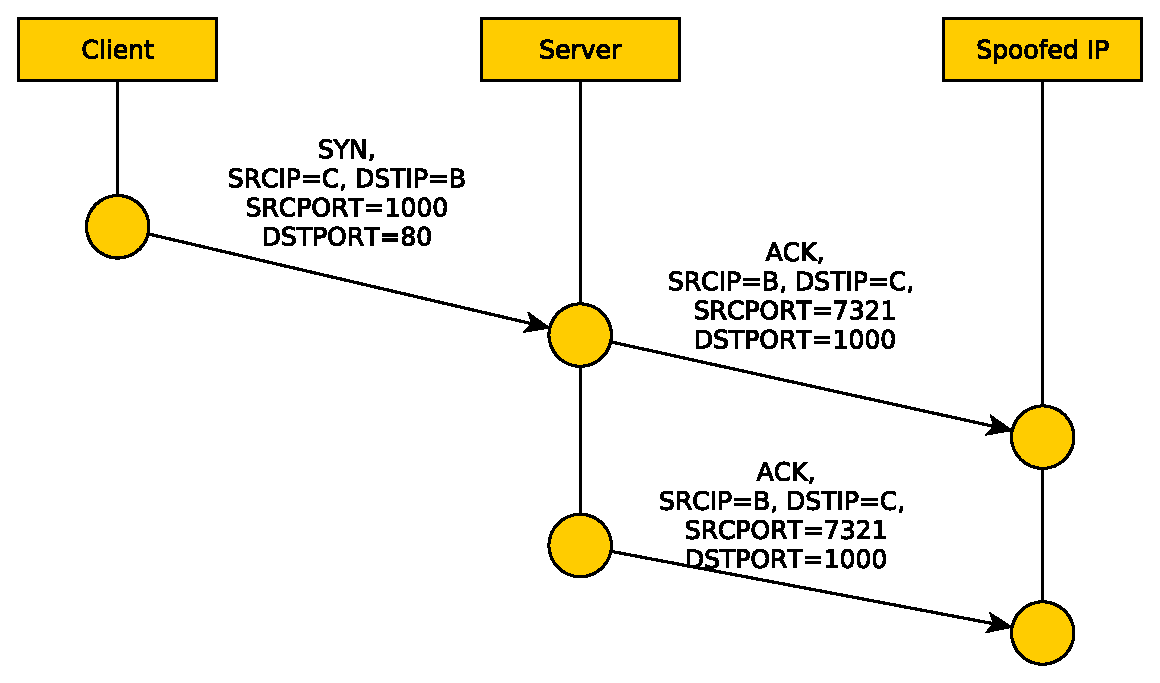
\includegraphics[width=0.8\linewidth]{syn2}
  \end{center}
  \begin{itemize}
  \item  Use non-existent C
  \item  Use C behind a dropping FW
  \item  Overload C
  \end{itemize}
\end{frame}


\begin{frame}{SYN Spoofing Attack }
  \begin{itemize}
  \item  attacker often uses either 
    \begin{itemize}
    \item  random source addresses 
    \item  or that of an overloaded server 
    \item  to block return of (most) reset packets 
    \end{itemize}
  \item  has much lower traffic volume 
    \begin{itemize}
    \item  attacker can be on a much lower capacity link 
    \end{itemize}
  \end{itemize}
\end{frame}


\begin{frame}{Types of Flooding Attacks }
  \begin{itemize}
  \item  classified based on network protocol used 
  \item  ICMP Flood 
    \begin{itemize}
    \item  uses ICMP packets, eg echo request 
    \item  typically allowed through, some required 
    \end{itemize}
  \item  UDP Flood 
    \begin{itemize}
    \item  alternative uses UDP packets to some port 
    \end{itemize}
  \item  TCP SYN Flood 
    \begin{itemize}
    \item  use TCP SYN (connection request) packets 
    \item  but for volume attack 
    \end{itemize}
  \end{itemize}
\end{frame}

\begin{frame}{Distributed Denial of Service Attacks }
  \begin{itemize}
  \item  have limited volume if single source used 
  \item  multiple systems allow much higher traffic 
    volumes to form a Distributed Denial of 
    Service (DDoS) Attack 
  \item  often compromised PC’s / workstations 
    \begin{itemize}
    \item  zombies with backdoor programs installed 
    \item  forming a botnet 
    \end{itemize}
  \item  e.g. Tribe Flood Network (TFN), TFN2K used a 
    trojan
  \end{itemize}
\end{frame}



\begin{frame}{DDoS Control Hierarchy}
  \begin{center}
    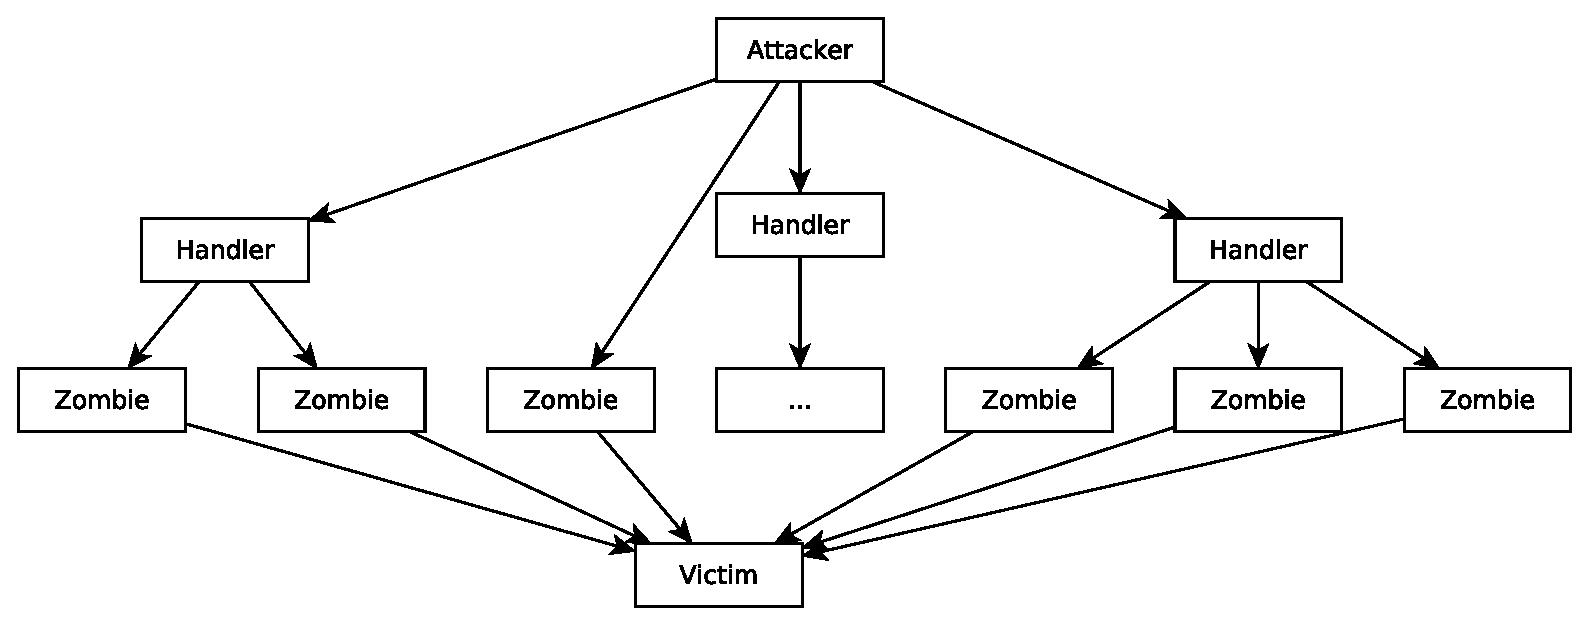
\includegraphics[width=1\linewidth]{ddos}
  \end{center}
\end{frame}

\begin{frame}{Connections}
  \begin{itemize}
  \item  (D)DoS – Malware – Countermeasures 
    (intrusion detection, firewalls, authentication) 
  \item  Risk to become a zombie 
  \item  Example: MyDoom 
    \begin{itemize}
    \item  Worm 
    \item  Backdoor 
    \item  DoS 
    \item  Blocking Antivirus
    \end{itemize}
  \end{itemize}
\end{frame}


\begin{frame}{Reflection Attacks}
  \begin{itemize}
  \item  use normal behavior of network 
  \item  attacker sends packet with spoofed source 
    address being that of target to a server 
  \item  server response is directed at target 
  \item  if send many requests to multiple servers, 
    response can flood target 
  \item  various protocols e.g. ICMP, UDP or TCP/SYN 
  \item  ideally want response larger than request 
  \item  prevent if block source spoofed packets
  \end{itemize}
\end{frame}



\begin{frame}{Reflection Attacks }
  \begin{itemize}
  \item  further variation creates a self-contained loop 
    between intermediary and target 
  \item  fairly easy to filter and block
  \end{itemize}
  \begin{center}
  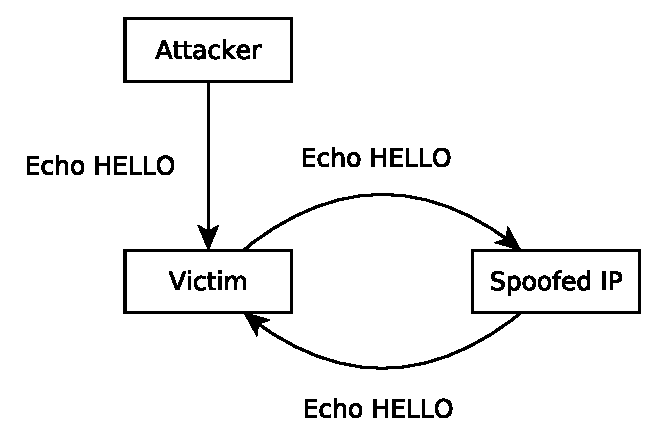
\includegraphics[width=0.6\linewidth]{reflection}
  \end{center}
\end{frame}

\begin{frame}{Amplification Attacks}
  \begin{center}
  \includegraphics[width=0.8\linewidth]{amplification}
  \end{center}
\end{frame}

\begin{frame}{DNS Amplification Attacks }
  \begin{itemize}
  \item  use DNS requests with spoofed source 
    address being the target 
  \item  exploit DNS behavior to convert a small 
    request to a much larger response 
    \begin{itemize}
    \item  60 byte request to 512 - 4000 byte response 
    \end{itemize}
  \item  attacker sends requests to multiple well 
    connected servers, which flood target 
    \begin{itemize}
    \item  need only moderate flow of request packets 
    \item  DNS servers will also be loaded 
    \end{itemize}
  \end{itemize}
\end{frame}



\begin{frame}{DoS on Phones}
  \begin{itemize}
  \item  See SMS-o-Death by Collin Mulliner 
  \item  http://www.mulliner.org/security/sms
  \end{itemize}
\end{frame}


\begin{frame}{SMTP}
  \begin{itemize}
  \item Mail reflection
  \begin{itemize}
  \item A sends: from: c@C to: b@B hello
  \item B sends: from: b@B to: c@C vacation message
  \item C sends: from: c@C to: b@B vacation message
  \end{itemize}
  \item<2-> Quota full
  \item<3-> User not allowed e.g. SMTP fax proxy
  \item<4-> Non existing user
  \end{itemize}
\end{frame}

\begin{frame}{ZIP}
  \begin{itemize}
  \item Infinite recursive zip: e.g. r.zip
  \item<2-> Bombs (e.g. non recursive files)    
    \begin{itemize}
      \item gzip: 100 GB, 97 MB compressed, 1000:1 ration
      \item bzip2: 100 GB, 69 KB, $1.6*10^6$:1
      \item PNG image: 19000 x 19000, 1-bit (45 MB) expand in 24-bit
        color to 1 GB, 44 KB compressed, 1000:1
    \end{itemize}
  \end{itemize}
\end{frame}

\begin{frame}[fragile]{XML}
  \footnotesize \begin{verbatim}
<?xml version="1.0"?>
<!DOCTYPE lolz [
 <!ENTITY lol "lol">
 <!ELEMENT lolz (#PCDATA)>
 <!ENTITY lol1 "&lol;&lol;&lol;&lol;&lol;&lol;&lol;&lol;&lol;&lol;">
 <!ENTITY lol2 "&lol1;&lol1;&lol1;&lol1;&lol1;&lol1;&lol1;&lol1;&lol1;&lol1;">
 <!ENTITY lol3 "&lol2;&lol2;&lol2;&lol2;&lol2;&lol2;&lol2;&lol2;&lol2;&lol2;">
 <!ENTITY lol4 "&lol3;&lol3;&lol3;&lol3;&lol3;&lol3;&lol3;&lol3;&lol3;&lol3;">
 <!ENTITY lol5 "&lol4;&lol4;&lol4;&lol4;&lol4;&lol4;&lol4;&lol4;&lol4;&lol4;">
 <!ENTITY lol6 "&lol5;&lol5;&lol5;&lol5;&lol5;&lol5;&lol5;&lol5;&lol5;&lol5;">
 <!ENTITY lol7 "&lol6;&lol6;&lol6;&lol6;&lol6;&lol6;&lol6;&lol6;&lol6;&lol6;">
 <!ENTITY lol8 "&lol7;&lol7;&lol7;&lol7;&lol7;&lol7;&lol7;&lol7;&lol7;&lol7;">
 <!ENTITY lol9 "&lol8;&lol8;&lol8;&lol8;&lol8;&lol8;&lol8;&lol8;&lol8;&lol8;">
]>
<lolz>&lol9;</lolz>
  \end{verbatim}
  \begin{itemize}
    \item 1 KB file
    \item 3GB XML (DOM worst)
  \end{itemize}
\end{frame}

\begin{frame}{Fork Bomb}
  \begin{itemize}
  \item PostgreSQL 7.2
  \item Uses elapsed milliseconds to compute number of thread to spawn
  \item No limit check
  \item<2-> What happen if you advance the date of one year?
  \item<3-> Network Time Protocol attack
 \end{itemize}
\end{frame}

\begin{frame}{Old SMS attack}
  \begin{itemize}
  \item Limited number of SMSs (i.e. 9) stored into the phone
  \item No limit in the reception from the provider
  \item Usage of zombie and Internet free SMS servers
  \item Fill and block the SMS reception of a user
 \end{itemize}
\end{frame}

\begin{frame}{HTTP}
  \begin{itemize}
  \item Distributed flood (spiders)
  \item Slashdotted
  \item Slowloris
  \begin{itemize}
    \item HTTP server: one thread/one request
    \item Open connection
    \item Infinitely (and slowly) send HTTP headers
    \item Consume the thread pool
  \end{itemize}
 \end{itemize}
\end{frame}

\begin{frame}{DoS Attack Defenses }
  \begin{itemize}
  \item  high traffic volumes may be legitimate 
    \begin{itemize}
    \item  result of high publicity, e.g. “slash-dotted” 
    \item  or to a very popular site, e.g. Olympics etc 
    \end{itemize}
  \item  or legitimate traffic created by an attacker 
  \item  three lines of defense against (D)DoS: 
    \begin{itemize}
    \item  attack prevention and preemption 
    \item  attack detection and filtering 
    \item  attack source traceback and identification
    \end{itemize}
  \end{itemize}
\end{frame}



\begin{frame}{Attack Prevention }
  \begin{itemize}
  \item  block spoofed source addresses 
    \begin{itemize}
    \item  on routers as close to source as possible (ingress filtering)
    \item  still far too rarely implemented 
    \item  alternatively enforce ``unicast severse path''
    \end{itemize}
  \item  rate controls in upstream distribution nets 
    \begin{itemize}
    \item  on specific packets types 
    \item  e.g. some ICMP, some UDP, TCP/SYN 
    \end{itemize}
  \item  use modified TCP connection handling 
    \begin{itemize}
    \item  use SYN cookies when table full (consumes computational resources)
    \item  or selective or random drop when table full 
    \end{itemize}
  \end{itemize}
\end{frame}

\begin{frame}{Attack Prevention }
  \begin{itemize}
  \item  block IP directed broadcasts 
  \item  block suspicious services (e.g. echo) \& combinations (DNS to
    echo port)
  \item  manage application attacks with “puzzles” to 
    distinguish legitimate human requests 
  \item  good general system security practices 
  \item  use mirrored and replicated servers when 
    high-performance and reliability required
  \end{itemize}
\end{frame}



\begin{frame}{Responding to Attacks }
  \begin{itemize}
  \item  need good incident response plan 
    \begin{itemize}
    \item  with contacts for ISP 
    \item  needed to impose traffic filtering upstream 
    \item  details of response process 
    \end{itemize}
  \item  have standard filters 
  \item  ideally have network monitors and IDS 
    \begin{itemize}
    \item  to detect and notify abnormal traffic patterns 
    \end{itemize}
  \end{itemize}
\end{frame}



\begin{frame}{Responding to Attacks}
  \begin{itemize}
  \item  identify type of attack 
    \begin{itemize}
    \item  capture and analyze packets 
    \item  design filters to block attack traffic upstream 
    \item  or identify and correct system/application bug 
    \end{itemize}
  \item  have ISP trace packet flow back to source 
    \begin{itemize}
    \item  may be difficult and time consuming 
    \item  necessary if legal action desired 
    \end{itemize}
  \item  implement contingency plan 
  \item  update incident response plan 
  \end{itemize}
\end{frame}



\begin{frame}{Summary}
  \begin{itemize}
  \item  introduced denial of service (DoS) attacks 
  \item  classic flooding and SYN spoofing attacks 
  \item  ICMP, UDP, TCP SYN floods 
  \item  distributed denial of service (DDoS) attacks 
  \item  reflection and amplification attacks 
  \item  defenses against DoS attacks 
  \item  responding to DoS attacks 
  \end{itemize}
\end{frame}

\end{document}




%%% Local Variables: 
%%% mode: latex
%%% TeX-master: t
%%% End: 
